\documentclass[conference]{IEEEtran}
\usepackage[spanish]{babel}
\usepackage[utf8]{inputenc}
\usepackage{blindtext, graphicx}
\usepackage{subfigure}
\usepackage{mdwmath}
\usepackage{mdwtab}
\usepackage{subfig}

\begin{document}
\title{ Suavizado de una imagen utilizando filtros de promedio y mediana. }
\author{\IEEEauthorblockN{Walter Alejandro Moreno Ram\'irez}
\IEEEauthorblockA{Departamento de Estudios Multidisciplinarios\\
Universidad de Guanajuato\\
Yuriria, Guanajuato\\
Correo: wa.morenoramirez@ugto.mx}}

\maketitle
\renewcommand\abstractname{Abstract}
\begin{abstract}
This article describes what is the meaning of local smoothing, the diferent methods that we can applied over an image such as the average filter and median filter. Also show their advantages as well as their applications. \\\\
\end{abstract}

\begin{IEEEkeywords}
Pixel, convoluci\'on, filtros, promedio, mediana, funci\'on, C++, OpenCV, ventana, m\'ascara.
\end{IEEEkeywords}

\IEEEpeerreviewmaketitle
\section{Introducci\'on} 
Para realizar mejoras y obtener informaci\'on de las im\'agenes existen distintos m\'etodos, las cuales se pueden categorizar de acuerdo a la transformaciones que realizas sobre la imagen o sobre su histograma.\\ Como se realiz\'o en pr\'acticas anteriores, se puede mejorar las caracter\'isticas de una imagen realizando transformaciones sobre su histograma. Tambi\'en se pueden obtener buenos resultados aplicando transformaciones sobre cada pixel, donde un pixel en la imagen de salida depende de la transformaci\'on que se le aplique al pixel en la misma posici\'on de la imagen de entrada.\\
Al aplicar dichos m\'etodos se obtienen resultados como en el aumento de contraste, correcci\'on de brillo, obtener negativos de la imagen, entre otros resultados posibles. Cada t\'ecnica o m\'etodo se realiza ya sea sobre el histograma o sobre un pixel en espec\'ifico. Para esta pr\'actica  se utilizar\'an m\'etodos en el dominio espacial.\\\\
\textbf{Dominio espacial\\}
El t\'ermino dominio espacial se refiere al conjunto de puntos que componen una imagen y los procedimientos en el dominio espacial operan directamente sobre los p\'ixeles. \\
Una transformaci\'on en el dominio espacial se puede expresar de acuerdo a la Ecuaci\'on (1).\\
\begin{equation}
	g(x,y) = T[f(x,y)]
\end{equation}

 donde $f(x,y)$ es la imagen de entrada, g(x,y) es la imagen procesada, y $T$ es el operador definido sobre alguna vecindad del punto $(x,y)$.\\\\ Para definir la vencidad de $(x,y)$ se utiliza una m\'ascara, matriz, filtro o subimagen con centro en el pixel ubicado en (x,y). Para esta pr\'actica se utilizar\'an matrices bidimensionales sim\'etricas que tengan por lado un valor impar, esto para que la matriz tenga un centro, a estas matrices se les llamar\'a filtro. El centro del filtro, que coincide con un pixel de la imagen, se mueve por toda la imagen, pixel a pixel, para as\'i obtener el valor de la nueva imagen g(x,y) en cada punto.

\section{Metodolog\'ia}
En una imagen digital, la convoluci\'on se denomina a una funci\'on que transforma la imagen de entrada en una nueva imagen de salida. La funci\'on de convoluci\'on se expresa por el s\'imbolo $\ast$.\\\\
La convoluci\'on entre una imagen $g(x,y)$ con respecto al filtro se denota en la Ecuaci\'on (2).\\\\
\begin{equation}
	f(i,j) = \sum\sum_{(x,y)\epsilon O} h(i-m,j-n)\ast g(m,n)
\end{equation}
Donde $f(i,j)$ es la imagen de salida, $h(i-m,j-n)$ es el vecindario del pixel central que coincide con el centro del filtro y $g(m,n)$ es la imagen de entrada, con estos dos \'ultimos factores denotamos la convoluci\'on entre la imagen y el filtro.\\ Las coordenadas $(i-m,j-n)$ representan la posici\'on donde nos ubicaremos dentro del filtro, esto debido a que es necesario desplazarse de la posici\'on del pixel central con coordenadas $(i,j)$, o lo que es lo mismo, nos desplazamos a la esquina superior izquierda de nuestro filtro, siendo $m$ y $n$ el radio o la distancia entre el pixel central con alguna orilla de nuestro filtro. Se realiza dicho desplazamiento para comenzar a recorrer todo el filtro, elemento a elemento y realizar las operaciones pertinentes.\\
Dichos filtros ser\'an matrices con valores de uno en todas sus posiciones. Si se quiere rezaltar un valor simplemente se agrega un valor mayor en la posici\'on deseada, comunmente el centro de nuestro filtro. Como ejemplo de un filtro se puede ver en la Figura 1.

\begin{figure}[h]
	\begin{center}
		\setlength{\unitlength}{0.00105in}
		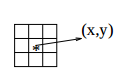
\includegraphics[scale=0.75]{./images/vecinos.png}
	\end{center}
	\caption{Filtro de dimensi\'on 3x3 con centro en $(x,y)$, donde $x$ son columnas y $y$ filas. }
\end{figure}

\newpage
\textbf{Filtro de promedio\\\\}
Para realizar un suavizado utilizando un filtro de promedio en una imagen primero se define el filtro con valores de 1 en todas sus posiciones. Se recorre la imagen pixel a pixel, la vecindad de cada pixel estar\'a dado por el tama\~no de nuestro filtro. \'Este m\'etodo implica obtener el promedio entre todos los vecinos del pixel central incluido este mismo, el resultado de la convoluci\'on para cada pixel ser\'a el valor para cada pixel individual en la imagen de salida. El promedio se obtiene sumando los valores de todos los p\'ixeles vecinos y el pixel central, dicha suma se dividir\'a entre la suma total de los valores del filtro. En la Figura 2. se muestra un filtro bidimensional de 3x3 con valor de 1 en todas sus posiciones.

\begin{figure}[h]
	\begin{center}
		\setlength{\unitlength}{0.00105in}
		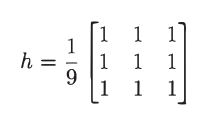
\includegraphics[scale=0.50]{./images/filtro.png}
	\end{center}
	\caption{Ejemplo de un filtro de promedio bidimensional de 3x3.}
\end{figure}

El procedimiento anteriormente explicado se representa mediante el pseudoc\'odigo de la Figura 3.\\

\begin{figure}[h]
	\begin{center}
		\setlength{\unitlength}{0.00105in}
		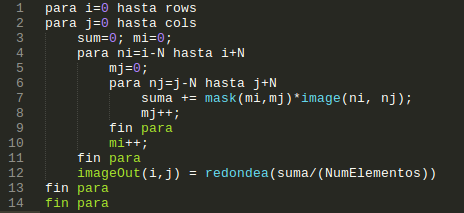
\includegraphics[scale=0.50]{./images/average.png}
	\end{center}
	\caption{Pseudoc\'odigo para realizar la convoluci\'on entre una imagen y un filtro de promedio.}
\end{figure}

Donde rows son las filas de la imagen, cols las columnas. suma es la variable encargada de acumular la suma para cada vecindad, $mi$ y $mj$ son contadores para poder ir cambiando de posici\'on dentro del filtro que tiene como nombre ``mask'', $ni$ y $nj$ ambos son contadores con las posiciones en que se mueve el filtro pero de la imagen de entrada. ``imageOut'' es el objeto creado para la imagen resultante de la convoluci\'on. ``NumElementos'' es el total de p\'ixeles dentro del filtro.\\
Se puede realizar la convoluci\'on de dos maneras distintas, primero se puede dividir cada elemento del filtro entre el total de elementos y posteriormente realizar la convolucu\'on con la imagen o primero se realiza la convoluci\'on y posteriormente se divide el valor total para obtener el promedio.\\\\ Cabe mencionar que, como el filtro tendr\'a valores fuera de las dimensiones de la imagen de entrada al posicionarse en las orillas de la misma, como resultado, el promedio tender\'a a un tono de gris muy oscuro, lo que se traduce en un marco con dichos tonos de gris alrededor de toda la imagen, el ancho del marco ser\'a proporcional al radio del filtro.\\
Para solucionar este imperfecto se pueden aplicar distintas t\'ecnicas como realizar un espejo con los valores de los p\'ixeles que se encuentre dentro de las dimensiones y realizar el promedio con dichos valores. Una manera m\'as sencilla es omitir esas posiciones exteriores y simplemente realizar el promedio con los valores v\'alidos para la imagen de entrada. Para \'esta pr\'actica se realiza la segunda t\'ecnica ya mencionada.\\\\

\textbf{Filtro de mediana\\\\}
Una vez que se tiene el filtro de promedio, el filtro de mediana es similar. Nos ubicamos en cada pixel de la imagen y obtenemos todos sus valores vecinos determinado por las dimensiones del filtro, y dichos valores se guardan en un vector o arreglo. Para esta pr\'actica se utiliz\'o una funci\'on a parte para ordenar de menor a mayor los valores dentro del filtro utilizando el m\'etodos de burbuja para el ordenamiento y escoger el valor que se encuentre en medio, para esto se divide el tama\~no de un lado del filtro entre dos. La funci\'on retorna el valor central que corresponde a la mediana del conjunto de valores contenidos en el filtro. Este procedimiento se realizar con todos los p\'ixeles de la imagen de acuerdo al pseudoc\'odigo de la Figura 4.

\begin{figure}[h]
	\begin{center}
		\setlength{\unitlength}{0.00105in}
		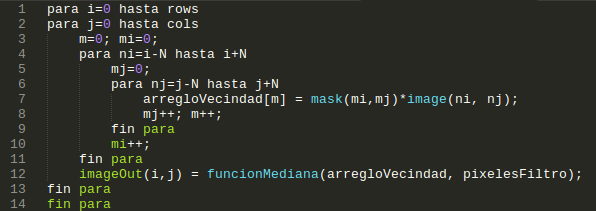
\includegraphics[scale=0.45]{./images/median.png}
	\end{center}
	\caption{Pseudoc\'odigo para realizar la convoluci\'on entre una imagen y un filtro de mediana.}
\end{figure}

Al igual que en la Figura 3. el pseucod\'ogio para el filtro de mediana es similar, la diferencia es que los valores resultantes de la convoluci\'on entre el filtro y la imagen se guardan en un arreglo ``arregloVecindad'' para al final de cada bucle asignar el valor medio o mediana obtenido de la funci\'on ``funcionMediana'' que se le pasan como par\'ametros tanto el arreglo como el total de elementos dentro del filtro.\\

\section{Resultados}
Se realizaron pruebas con tres im\'agenes en total, dos para la convoluci\'on con el filtro de promedio y una para la convoluci\'on entre el filtro de mediana.\\
Las im\'agenes que se utilizaron para las pruebas se pueden observar en la Figura 5.

\begin{figure}[htbp]
	\centering
	\subfigure[]{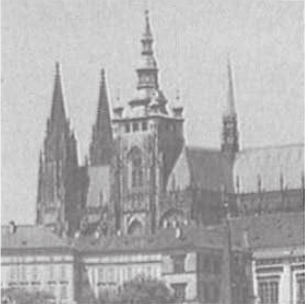
\includegraphics[scale=0.28]{./images/castle.png}}
	\subfigure[]{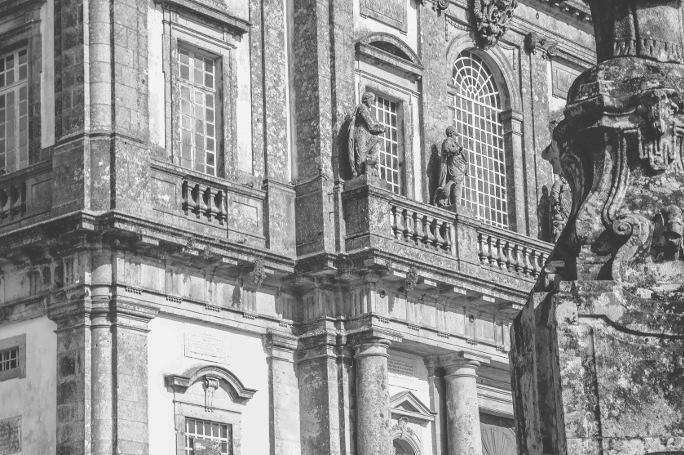
\includegraphics[scale=0.25]{./images/house.jpg}}
	\subfigure[]{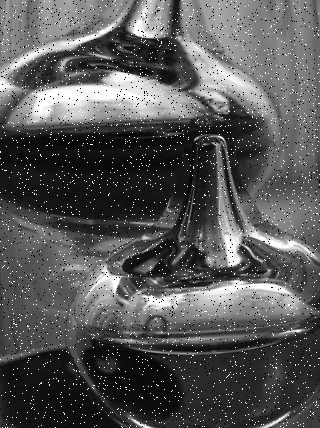
\includegraphics[scale=0.2517]{./images/noise1.png}}
	\caption{(a) y (b) se utilizaron para la convoluci\'on con el filtro de promedio; (c) para la convoluci\'on con el filtro de mediana. }
\end{figure}

\textbf{ Filtro de promedio (pruebas y resultados):\\\\}
Cuando se realiz\'o la convoluci\'on entre la imagen y el filtro de promedio con la imagen de la Figura 5. (a) el resultado se muestra en la figura 6.

\begin{figure}[htbp]
	\centering
	\subfigure[Imagen de entrada]{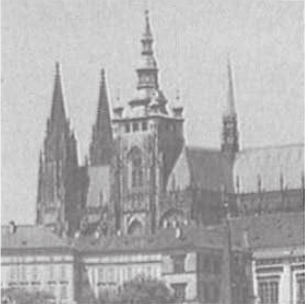
\includegraphics[scale=0.37]{./images/castle.png}}
	\subfigure[Imagen de salida]{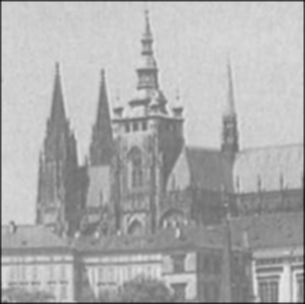
\includegraphics[scale=0.494]{./images/castleOut3x3}}
	\caption{Convoluci\'on aplicando un filtro de promedio de 3x3.}
\end{figure}

\newpage
De la Figura 6. podemos observar un suavizado ligero ya que es un filtro peque\~no, lo que se hace notar m\'as es el recuadro negro que es el resultado de dicho filtro, de igual manera, no es tan notorio.\\\\
Cuando notamos una diferencia sustancial es al realizar la convoluci\'on con un filtro de 7x7 como se muestra en la Figura 7.

\begin{figure}[h]
	\centering
	\subfigure[Imagen de entrada]{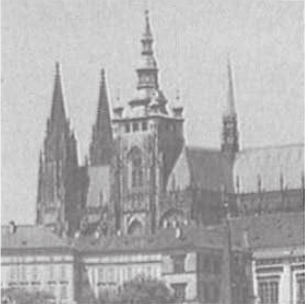
\includegraphics[scale=0.37]{./images/castle.png}}
	\subfigure[Imagen de salida]{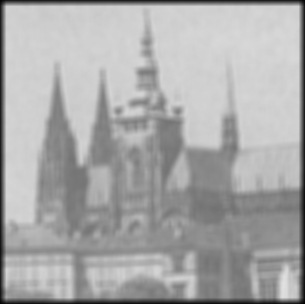
\includegraphics[scale=0.494]{./images/castleOut7x7}}
	\caption{Convoluci\'on aplicando un filtro de promedio de 7x7.}
\end{figure}

La imagen de salida es incluso a\'un mas suavizada, llegando a un punto donde se pierdes algunos detalles como las ventanas del castillo o se mezclan sombras de los tejados.\\
Tambi\'en se puede apreciar un marco de un tono de gris muy oscuro debido a la gran cantidad de p\'ixeles con dicho tono de gris que se encuentran en las orillas al momento del filtro coincidir con los p\'ixeles de las orillas. Su grosor tambi\'en se ve aumentado debido al taman\~o del filtro.\\

Para la segunda imagen, al aplicar el mismo procedimiento con un filtro de 3x3 el suavizado se nota poco, aunque est\'a presente como se muestra en la Figura 8.\\

\begin{figure}[h]
	\centering
	\subfigure[Imagen de entrada]{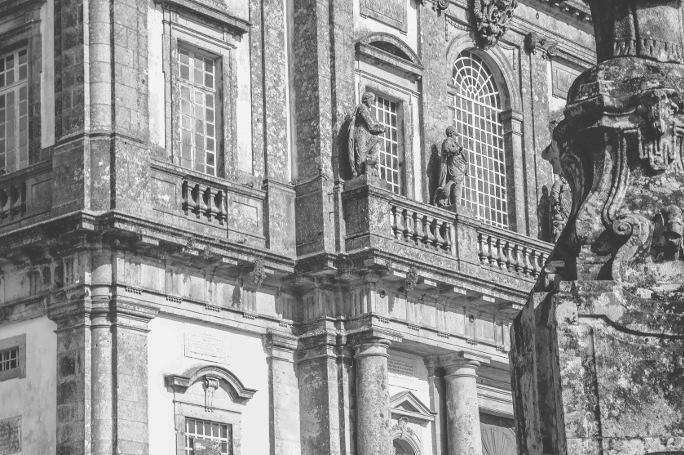
\includegraphics[scale=0.25]{./images/house.jpg}}
	\subfigure[Imagen de salida]{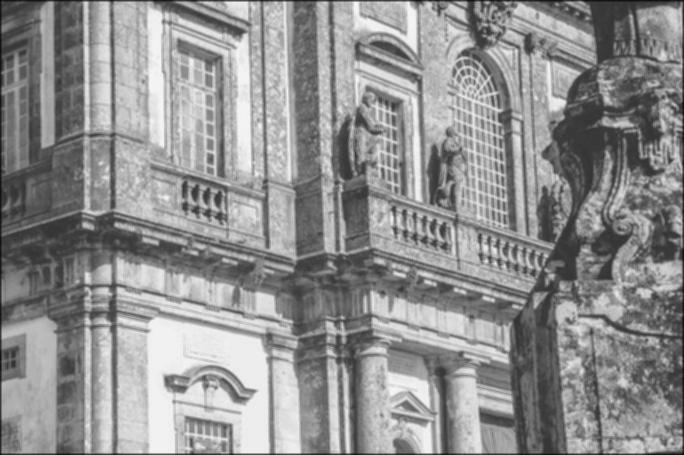
\includegraphics[scale=0.25]{./images/houseOut3x3.jpg}}
	\caption{Convoluci\'on aplicando un filtro de promedio de 3x3.}
\end{figure}

Al tener tonos de grises muy oscuros en las orillas de la imagen el marco negro caracter\'istico de estos filtros no es muy notorio.\\
Todo cambia cuando se aumenta de tama\~no al filtro, pasando a ser de 7x7 lo que tiene repercusiones en la imagen de salida dandole un suavizado m\'as marcado y notorio. Al igual, el marco se hace presente ya que aumenta de grosor, esto se aprecia mejor en la Figura 9.

\begin{figure}[h]
	\centering
	\subfigure[Imagen de entrada]{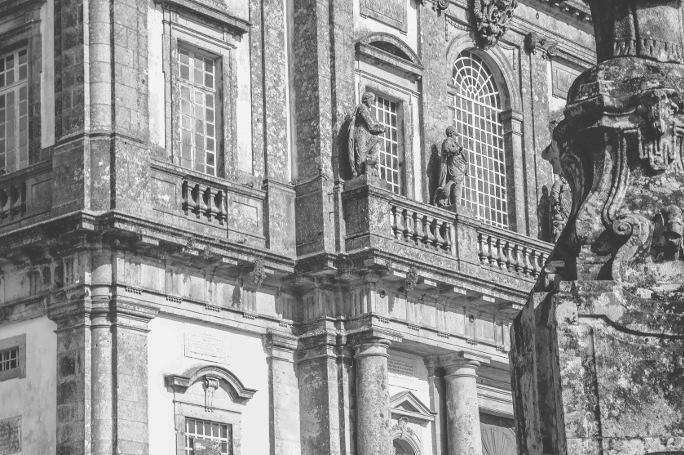
\includegraphics[scale=0.25]{./images/house.jpg}}
	\subfigure[Imagen de salida]{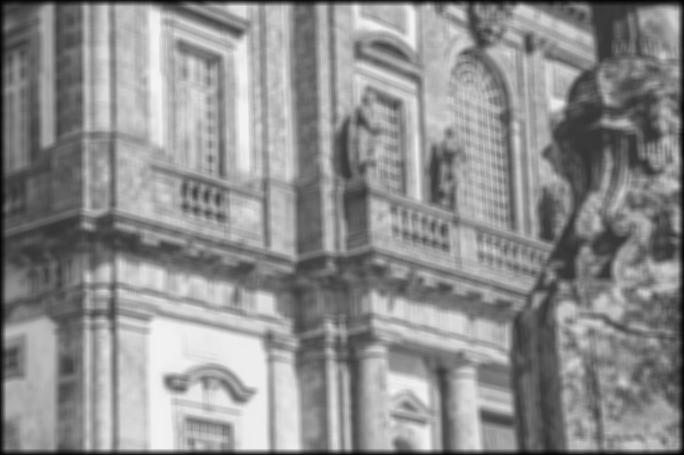
\includegraphics[scale=0.25]{./images/houseOut7x7.jpg}}
	\caption{Convoluci\'on aplicando un filtro de promedio de 7x7.}
\end{figure}

\textbf{ Filtro de promedio (pruebas y resultados):\\\\}
Al realizar la convoluci\'on con el filtro de mediana los cambios son muy distintos. Debido al procedimiento para obtener el valor en cada pixel de la imagen de salida, en este caso se realiza utilizando el valor que se encuentre en medio de un arreglo de los valores vecinos del pixel central.\\
Obtener la mediana de un conjunto de valores es \'util al momento de quere eliminar el ruido de una imagen, mas exactamente el ruido del tipo sal y pimienta como se muestra en la Figura 10.

\begin{figure}[h]
	\centering
	\subfigure[Imagen de entrada]{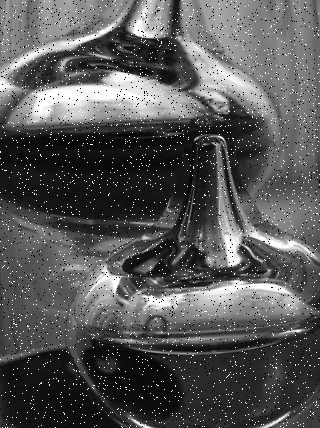
\includegraphics[scale=0.30]{./images/noise1.png}}
	\subfigure[Imagen de salida]{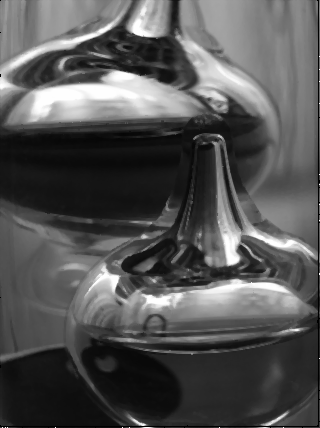
\includegraphics[scale=0.40]{./images/noise1Out3x3}}
	\caption{Convoluci\'on aplicando un filtro de mediana de 3x3.}	
\end{figure}
\newpage
Pero si el filtro aumenta de tama\~no, la imagen de salida comienza a perder detalle. Los tonos grises claros se comienzan a mezclar con los tonos grises medios y grises oscuros viendose de mejor manera en la Figura 11.

\begin{figure}[h]
	\centering
	\subfigure[Imagen de entrada]{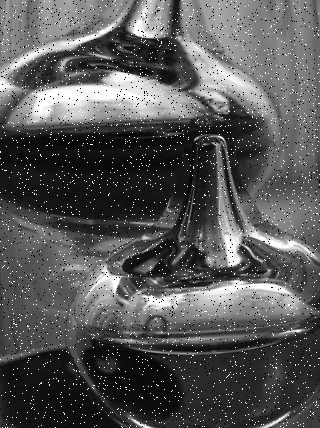
\includegraphics[scale=0.30]{./images/noise1.png}}
	\subfigure[Imagen de salida]{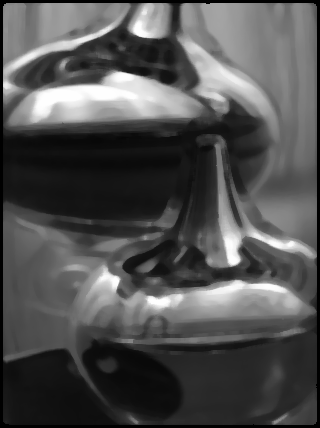
\includegraphics[scale=0.40]{./images/noise1Out7x7}}
	\caption{Convoluci\'on aplicando un filtro de mediana de 7x7.}	
\end{figure}

Adem\'as, al aumentar el taman\~no del filtro, lo que implica que en las orillas se encuentren con una mayor cantidad de tonos negros, se comienza a observar un recuadro negro en toda la imagen. Conforme el taman\~no del filtro va aumentando tambi\'en se notar\'a m\'as el recuadro negro en cualquier imagen.\\\\
Los resultados de realizar la convoluci\'on con un filtro de mediana son buenos mientras no exista mucho ruido en la imagen, ya que al presentarse con menos diferencia entre p\'ixeles, la mediana seguir\'a siendo, en algunos casos, un valor que corresponda al ruido presente en la imagen.\\\\

\section{Conclusiones}
Es importante escoger un tama\~no adecuado de nuestro filtro para cada imagen o un conjunto de im\'agenes semenjantes, ya que el escoger un filtro de tama\~no inadecuado puede causar la perdida de informaci\'on en las im\'agenes. Este detalle se puede reducir en gran medida resaltando los p\'ixeles importantes, esto se podr\'ia realizar modificando los valores del filtro.\\
Para lograr el suavizado ideal se debe obtener una perfecta combinaci\'on entre la eliminaci\'on del ruido, y un suavizado tal que no se pierda informaci\'on de la imagen.

%\begin{thebibliography}{1}
%    \bibitem{IEEEhowto:kopka}
%    H.~Kopka and P.~W. Daly, \emph{A Guide to \LaTeX}, 3rd~ed.\hskip 1em plus
%      0.5em minus 0.4em\relax Harlow, England: Addison-Wesley, 1999.
%\end{thebibliography}

%\begin{IEEEbiography}[{\includegraphics[width=1in,height=1.25in,clip,keepaspe%ctratio]{picture}}]{John Doe}
%\blindtext
%\end{IEEEbiography}

\end{document}